%
\renewcommand{\theequation}{\theenumi}
\begin{enumerate}[label=\thesection.\arabic*.,ref=\thesection.\theenumi]
\numberwithin{equation}{enumi}
\numberwithin{figure}{enumi}
\numberwithin{table}{enumi}


\item निम्न बिंदु किस चतुर्भुज के शीर्ष हैं? कारण सहित अपने उत्तर की पुष्टि करें ।
\begin{align}
\vec{P} = \myvec{-1\\-2}, \vec{Q} =\myvec{1\\0},
\vec{R} =\myvec{-1\\2}, \vec{S} =\myvec{-3\\0}
\end{align}
\solution
आकृति 	\ref{fig:3.5.4_quadrilateral1} में
\begin{align}
\label{eq:constr_vectors_quad1_PSQR}
 \vec{P} - \vec{S} &= 
 \vec{Q} - \vec{R} = \myvec{2\\-2}
\\
\vec {R} - \vec {S} &=
 \vec {Q} - \vec {P} = \myvec{2\\2}
\label{eq:constr_vectors_quad1_RSQP}
\end{align}
%
$PQRS$ की सम्मुख भुजायें  समांतर हैं । अतः वह एक समांतर चतुर्भुज है । इसके अतिरिक्त
\begin{align}
\norm{ \vec{P} - \vec{S}} &= 
\norm{ \vec{Q} - \vec{R}} 
\\
=\norm{\vec {R} - \vec {S}} &=
\norm{ \vec {Q} - \vec {P}} = 2\sqrt{2}
\end{align}
%
$\because$ चतुर्भुज कीे समस्त भुजायें समान हैं, समांतर चतुर्भुज एक समचतुर्भुज है ।   $PS$ एवं
$RS$ से कृत कोण
\begin{align}
\cos \theta = \frac{\brak{\vec{S}-\vec{P}}^{\top}\brak{\vec{S}-\vec{R}}}{\norm{\vec{S}-\vec{P}}^{\top}\norm{\vec{S}-\vec{R}}}
\end{align}
%
$\because $
\begin{align}
\brak{\vec{S}-\vec{P}}^{\top}\brak{\vec{S}-\vec{R}} = \myvec{2 & -2}\myvec{2\\2} = 0
\end{align}
उपरोक्त समीकरण में $^{\top}$ अदिश गुणनफल का चिन्ह है.
\eqref{eq:constr_vectors_quad1_PSQR} का  \eqref{eq:constr_vectors_quad1_RSQP} में प्रतिस्थापन पर
\begin{align}
\cos \theta = 0 \implies PS \perp RS
\end{align}
%
अतः समचतुर्भुज मूलतः एक वर्ग है। 
\begin{figure}[!ht]
	\centering
	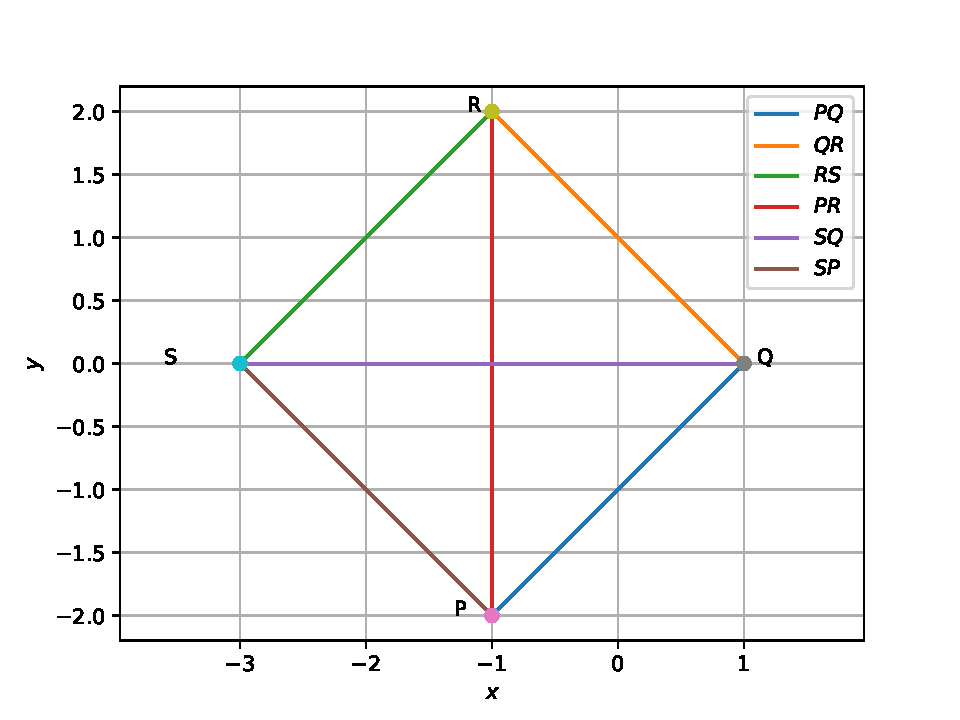
\includegraphics[width=\columnwidth]{figs/quad1.pdf}
	\caption{प्रदत्त बिंदुओं से एक वर्ग का निर्माण होता है।}
	\label{fig:3.5.4_quadrilateral1}
\end{figure}


\end{enumerate}

%\end{document}


